\documentclass[a4paper]{article}
\usepackage{amsmath,amssymb,enumerate, graphicx,amsfonts, makeidx, hyperref}
\usepackage{listings}
\lstset{language=C}
\begin{document}
\begin{center}

{\bf{\huge CS 225 }}\\
\vspace{ 0.5 cm }
{\bf{\huge a.k.a. }}\\
\vspace{ 0.5 cm }
{\bf{\huge Data Structures }}\\
\vspace{ 5 cm }
{\bf{\large Spring 2011}}\\
{\bf{\large University of Illinos}}\\
{\bf{\large as taught by Cynda Heer}}\\
\vspace{ 5 cm }                         
{\large notes by Michele R. Esposito}\\
\vspace{ 5cm }
Please, let report any error or type-o at\\
\underline{\href{mailto:micheleresposito@gmail.com}{ micheleresposito@gmail.com }}
\end{center}
\newpage
\tableofcontents
\newpage

% =========================================================

\section{Linear Data Structures} % (fold)
\label{sec:Linear Data Structures}
\subsection{Linked Lists} % (fold)
\label{sub:Linked Lists}
\begin{tabular}{ | c | c | c |}
  \hline
  {\bf Operations } & {\bf Running Time} & {\bf Notes}  \\
  \hline
  Insert front  & O(1) & \\
  \hline
  Insert back   & O(n) & O(1) in DLL w Sentinel node \\
  \hline
  Insert random  & O(n) & \\
  \hline
  Delete random  & O(n) & O(1) in double linked list \\
  \hline
  Lookup  & O(n) & \\
  \hline
\end{tabular} \\

Linked lists are a very simple data structure, which is a building block for many other data structures, like trees. There are two common types of Linked lists: {\bf Singly linked(SLL)} and {\bf double linked (DLL)}. SLL allows you to traverse only in one direction, whereas DLL allows you to traverse both ways.  \\
A {\bf Sentinel Node} is an empty node that is used to keep track of a certain location inside a linked list. They are usually positioned at the beginning and at the end of the list in order to speed up insertion and removal. \\
{\bf Disadvantages:} Linked list are usually very slow, as they are not stored contiguously in memory. In order to access the elements, you need to dereference all the pointers, which can be very slow. \\
{\bf Advantages:} Its useful to use linked list if you know that you will be moving your data around a lot, as its easy to rearrange them, without needing additional space. There are some versions of Malloc which are implemented using linked lists.
% subsection Linked Lists (end)
\subsection{Stack and Queues} % (fold)
\label{sub:Stack and Queues}
\begin{tabular}{ | c | c | c |}
  \hline
  {\bf Operations } & {\bf Running Time} & {\bf Notes}  \\
  \hline
  Pop & O(1) & Dequeue in queues \\
  \hline
  Push & O(1) & Enqueue in queues \\
  \hline
\end{tabular} \\
Stack and queues are two simple, yet very useful, data structures. Stacks are FILO, First In Last Out data structures, whereas queues are FIFO, First In/First Out. Both stacks and queue are usually implemented either using arrays, or using linked lists. Either way, a constant runtime is guaranteed for the above operations.\\
{\bf Implementation:} Implementing both a stack and a queue using a Linked List(LL) is straight forward. In the stack, you only need to keep of the top element, which is easy to do if you use a sentinel node. In a queue, you need to keep track of the first and last node, again easy to do if you use sentinel nodes.\\
Arrays are slightly more complicated, as you have the problem of filling up the array. Typically, when you fill up the array, you double the size and then copy the elements over. This operation will still give you an amortized time of $O(1)$ per insert. In a stack, you simply need to keep track of the position of the top element, then resize if the length of the array is equal to the index of the top element. \\ 
If you want to implement a queue using an array, then you need to keep track of the entry point and the exit point.\\
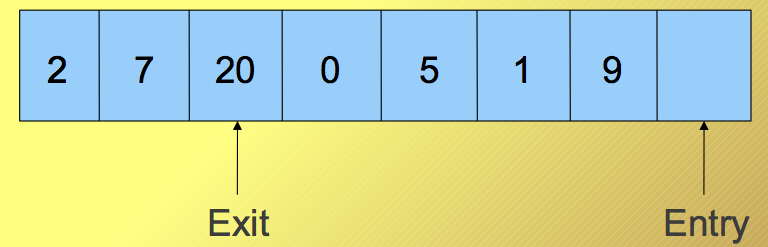
\includegraphics[scale=.40]{queueArray.png}\\
However, this time you resize only if $abs( exitPoint - entryPoint ) >= n$ where $entryPoint$, $exitPoint$ are indexes, and $n$ is the length of the array. This is because your indexes can cirulate thought the array.\\
{\bf Notes:} You can actually implement a queue using two stacks. The trick, is using one of the stacks enqueue elements, and the other to dequeue. Whenever you want to dequeue an element, simply reverse every other element inside the other stack, and you will be able to dequeue elements from there. 
% subsection Stack and Queues (end)
% section Linear Data Structures (end)
\section{Trees} % (fold)
\label{sec:Trees}
A tree is one of the most used data structures in CS, and its indeed very useful. There are many different kinds of tree, for all sort of purposes. In here, I will be covering some of the most common ones.
\subsection{Binary Search Tree} % (fold)
\label{sub:Binary Search Tree}
\begin{tabular}{ | c | c | c |}
  \hline
  {\bf Operations } & {\bf Average Case} & {\bf Worst case}  \\
  \hline
  Insert & O(log n) & O(n)\\
  \hline
  Removal & O(log n) & O(n) \\
  \hline
  Lookup & O(log n) &O(n)  \\
  \hline
\end{tabular} \\

A binary search tree (BST) is one of the simplest basic trees. It is defined in this way:\\
$ T = \{\} $ or \\
$ T = \{r , T_r, T_l\}$ where \\
$\forall$ $keys \in T_r \geq key(r)$ and $ \forall$ $keys \in T_l < key(r)$.\\
{\bf Advantages:} BST are straight forward to implement, and have a good average case $O(log n)$. They are good if you already know the median of the data that you are going to insert inside the tree. Like that, you can use the median value as root for your tree. Otherwise, you will run into an imbalanced tree.\\
{\bf Disadvantages:} BST do not guarantee height $\log n$. Say, for example, if you were going to insert elements from 1 to 10 in this order. Then, you would get a tree of height 10, which is bad news, because its just a fancy linked list. Thus, \emph{ the height is dependent on insert order}.
% subsection Binary Search Tree (end)
% \subsection{AVL Trees} % (fold)
% \label{sub:AVL Trees}
% 
% % subsection AVL Trees (end)
% \subsection{Red-Black trees} % (fold)
% \label{sub:Red-Black trees}
% 
% % subsection Red-Black trees (end)
% % section Trees (end)
\end{document}
